\documentclass[12pt]{article}
\usepackage{listings}
\usepackage[margin=1in]{geometry}
\usepackage{amsmath}
\usepackage{tikz}
\usetikzlibrary{shapes.geometric}
\usetikzlibrary{positioning}

\lstset{
  frame=leftline,
  numbers=left,
  language=C++,
  basicstyle=\footnotesize\ttfamily,
  breaklines=true
}
\begin{document}
\tableofcontents
\section{Data Structures}
\subsection{Binary Search Tree(BST).}
In a BST a node will always have a greater or smaller key than its left and
right child respectively.
\begin{figure}[!ht]
  \centering
  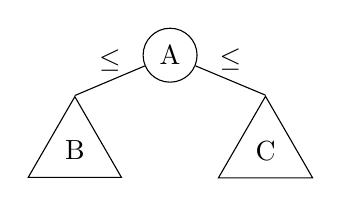
\begin{tikzpicture} [
    tree/.style = {draw, regular polygon, regular polygon sides=3 },
    node/.style = {draw, circle}
    ]
    \node[node] (A) {A};
    \node[tree, below left=1cm of A] (B) {B};
    \node[tree] (C) [below right=1cm of A] {C};

    \path (A) edge [above] node {$\leq$} (B.north);
    \path (A) edge [above] node {$\leq$} (C.north);
  \end{tikzpicture}
  \caption{BST}
\end{figure}

\noindent\begin{minipage}{\linewidth}
\lstinputlisting[firstline=6, lastline=17,
  title=Type definition]{BST.cpp}
\end{minipage}

\noindent\begin{minipage}{\linewidth}
\lstinputlisting[firstline=72, lastline=80,
  title=Insertion $O(h)$]{BST.cpp}
\end{minipage}
Inserting will travel the BST until it finds a null node to place the new value.
When the BST is not balanced the height $h$ can be at most the number of
nodes $n$.

\noindent\begin{minipage}{\linewidth}
\lstinputlisting[firstline=24, lastline=28,
  title=Minimum Node $O(h)$]{BST.cpp}
\end{minipage}
Allows to find the element with minimum key by moving only leftward down the
tree. Implementation for finding the maximum key is analogous.\\

\noindent\begin{minipage}{\linewidth}
\lstinputlisting[firstline=84, lastline=100,
  title=Removal $O(h)$]{BST.cpp}
\end{minipage}
When removing nodes there are 2 cases.\\
1: The node to remove has 1 or no children, so its child (the null node in case
of none) is going to take its place.\\
2: It has 2 nodes, in which case it is replaced by the least node in its right
subtree.\\

\noindent\begin{minipage}{\linewidth}
\lstinputlisting[firstline=40, lastline=52,
  title=Successor $O(h)$]{BST.cpp}
\end{minipage}
It also allows to find the successor of a number $n$ in the tree(least key
greater than $n$). Implementation for finding predecessor is analogous.\\

\noindent\begin{minipage}{\linewidth}
\lstinputlisting[firstline=104, lastline=110,
  title=Sorting $O(n)$]{BST.cpp}
\end{minipage}
Making an in-order traversal of a BST produces an ordered list of its
elements.\\

\subsection{AVL} 
\subsubsection{Union-Find Disjoint Sets}
\noindent\begin{minipage}{\linewidth}
\lstinputlisting[firstline=19, lastline=25,
  title=build $O(n)$ ]{unionFind.cpp}
\end{minipage}
Initializes each value as member of its own set

\noindent\begin{minipage}{\linewidth}
\lstinputlisting[firstline=27, lastline=29,
  title=build $\approx O(1)$]{unionFind.cpp}
\end{minipage}
Tells the set $a$ belongs to.

\noindent\begin{minipage}{\linewidth}
\lstinputlisting[firstline=31, lastline=43,
  title=merge $\approx O(1)$]{unionFind.cpp}
\end{minipage}
Merge the sets in which $a$ and $b$ belong to.

\subsection{Trees}
\subsubsection{Segment Tree}

\noindent\begin{minipage}{\linewidth}
\lstinputlisting[firstline=7, lastline=19,
  title=build $O(n)$]{segmentTree.cpp}
\end{minipage}
Stores the values of \textit{arr} in \textit{tree}, each node stores the
operation on a different interval of values. Root of \textit{tree} is 1.

\noindent\begin{minipage}{\linewidth}
\lstinputlisting[firstline=21, lastline=29,
  title=query $O(\log n)$]{segmentTree.cpp}
\end{minipage}
Returns the given operation on the range $[a, b]$.

\noindent\begin{minipage}{\linewidth}
\lstinputlisting[firstline=31, lastline=40,
  title=update $O(n)$]{segmentTree.cpp}
\end{minipage}
Increments every value in the range $[a, b]$ in $p$ units,
can be modified to change all values in the range to $p$ by changing
increment operator by assignation.

\noindent\begin{minipage}{\linewidth}
\lstinputlisting[firstline=26, lastline=35,
  title=propagate $O(1)$]{segmentTreeLazyProp.cpp}
\end{minipage}
Updates the value on \textit{node} and propagates
the lazy value to its children.

\noindent\begin{minipage}{\linewidth}
\lstinputlisting[firstline=37, lastline=51,
  title=lazy update $O(\log n)$]{segmentTreeLazyProp.cpp}
\end{minipage}
Increments every value in the range $[a, b]$ in $p$ units, lazy values
are stored in \textit{lazy}, updates on demand.

\noindent\begin{minipage}{\linewidth}
\lstinputlisting[firstline=53, lastline=62,
  title=lazy query $O(\log n)$]{segmentTreeLazyProp.cpp}
\end{minipage}
Computes the value of the operation in the range $[a, b]$, updates on demand.

\section{Graphs}
\subsection{MST}
\subsubsection{Kruskal}
\noindent\begin{minipage}{\linewidth}
\lstinputlisting[firstline=18, lastline=29,
  title=Kruskal $O(|E|\log |V|)$]{kruskal.cpp}
\end{minipage}
Computes the Minimum Spanning Tree of a graph with $E =$ \textit{edges}.

\subsection{SSSP}
\subsubsection{Dijkstra}

\noindent\begin{minipage}{\linewidth}
\lstinputlisting[firstline=10, lastline=32,
  title=Dijkstra $O(|E|+|V|\log |V|)$]{dijkstra.cpp}
\end{minipage}
Computes the shortest distance $d[u]$ from vertex $s$ to every vertex $u$,
stops after finding min distance to $e$.

\section{Math}
\subsection{Series}
\subsubsection{Aritmetic Progression}
\begin{align*}
  S_n &= a_1 + (a_1+d) + (a_1+2d) + \cdots + (a_1+(n-1)d)\\
  S_n &= \frac{n}{2}(2a_1+(n-1)d)
\end{align*}
\end{document}
